\documentclass[11pt]{article}
\usepackage[utf8]{inputenc}
\usepackage[brazilian]{babel}
\usepackage{graphicx}
\usepackage[a4paper, top={.4in}, bottom={.65in}]{geometry}
\usepackage{subfig}
\usepackage{makecell}
\usepackage{textcomp}
\usepackage{gensymb}
\usepackage{tikz}
\usepackage{amsmath}
\usepackage{amssymb}
\usepackage{upgreek}

\begin{document}

\begin{center}
  \textbf{Experimento 08 -- PSI-3212} \\
  Natanael Magalhães Cardoso, nUSP: 8914122
\end{center}

\subsection*{Item 1.a}

\begin{figure}[h!]
  \centering
  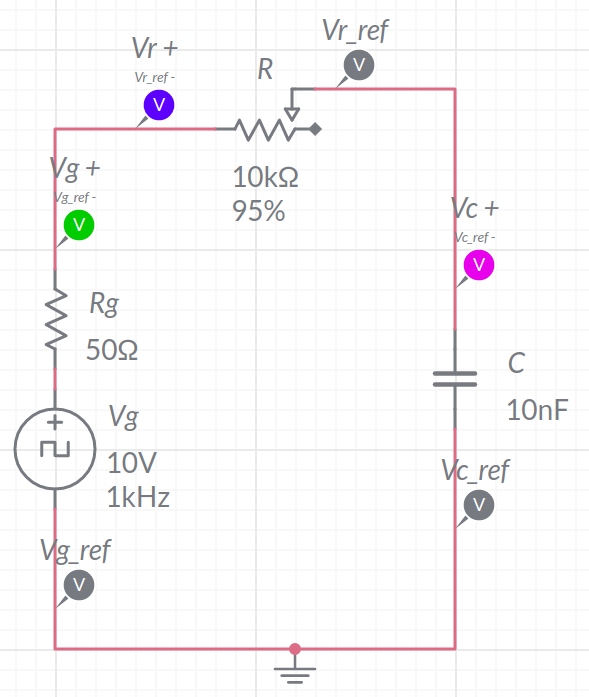
\includegraphics[width=.56\textwidth]{fig/1-circ}
  \caption{Esquema do circuito.}
  \label{fig:1-circ}
\end{figure}

\begin{figure}[h!]
  \centering
  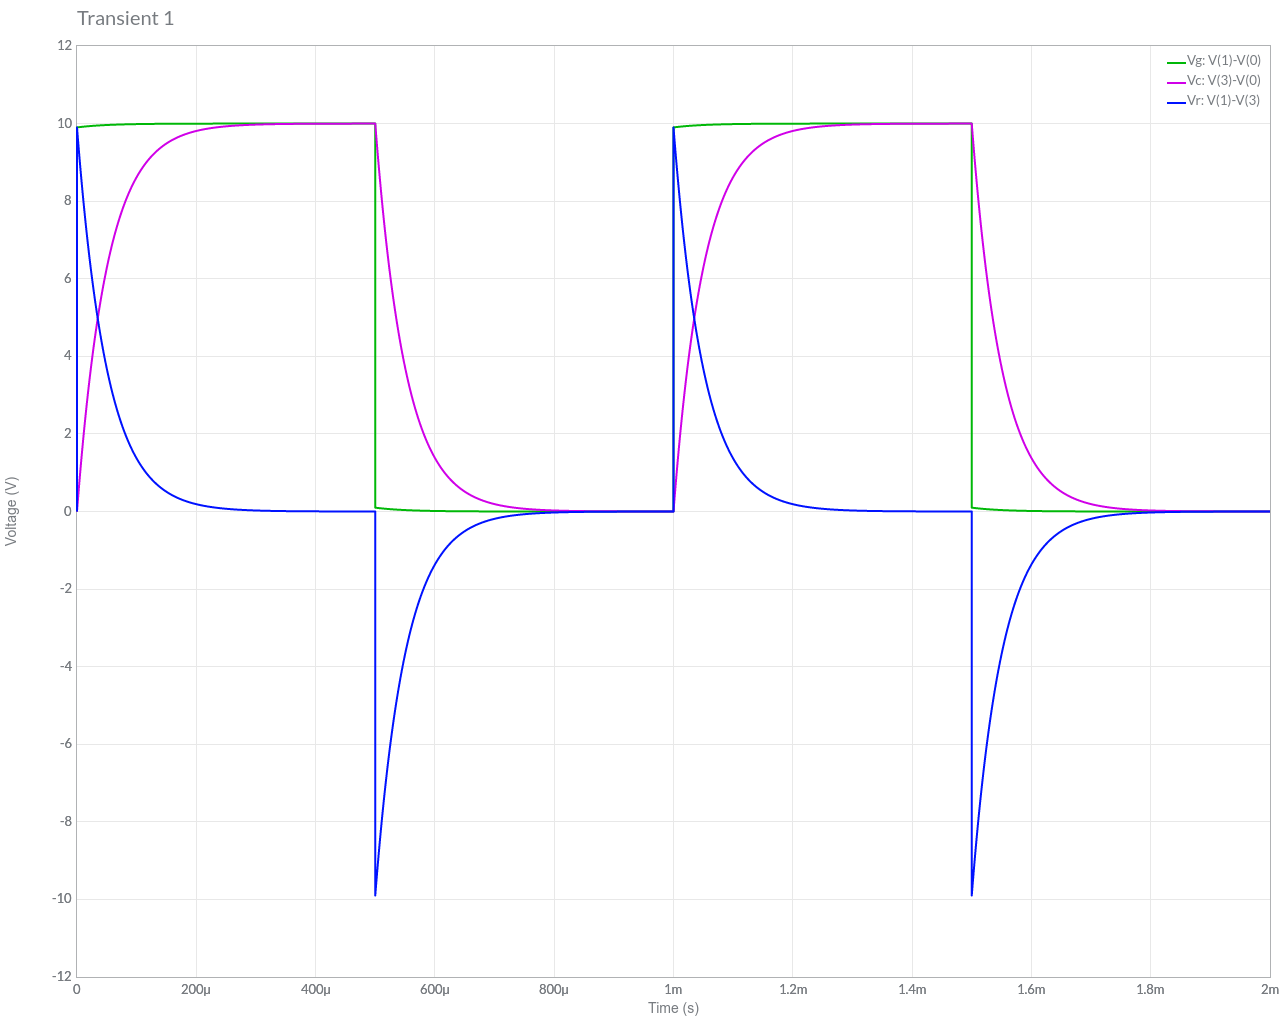
\includegraphics[width=.9\textwidth]{fig/1-sim}
  \caption{Simulação da circuito da figura \ref{fig:1-circ}.}
  \label{fig:1-sim}
\end{figure}


\subsection*{Item 1.b}

Observando a figura \ref{fig:1-sim} vemos que, no início, a tensão no capacitor é mínima enquanto a tensão no resistor é máxima e, no decorrer do tempo, a tensão no capacitor aumenta e a tensão no resistor diminui.

O formato da curva da tensão no capacitor no domínio do tempo é uma exponencial com uma assíntota em E, como esperado teoricamente.

\begin{equation}
  v_{c}(t) = E(1 - e^{-\frac{t}{\uptau}})
  \label{eq:vc-1}
\end{equation}

Pela segunda lei de Kirchhoff:

\begin{equation}
  E - v_{r} - v_{c} = 0 \, \overset{(\ref{eq:vc-1})}{\Rightarrow} \, v_{r} = E - E(1 - e^{-\frac{t}{\uptau}}) = -Ee^{\frac{t}{\uptau}}
  \label{eq:vr-1}
\end{equation}

Pela equação \ref{eq:vr-1}, é notado que a curva da tensão no resistor também possui uma forma esperada.

\subsection*{Item 1.c}

\begin{figure}[h!]
  \centering
  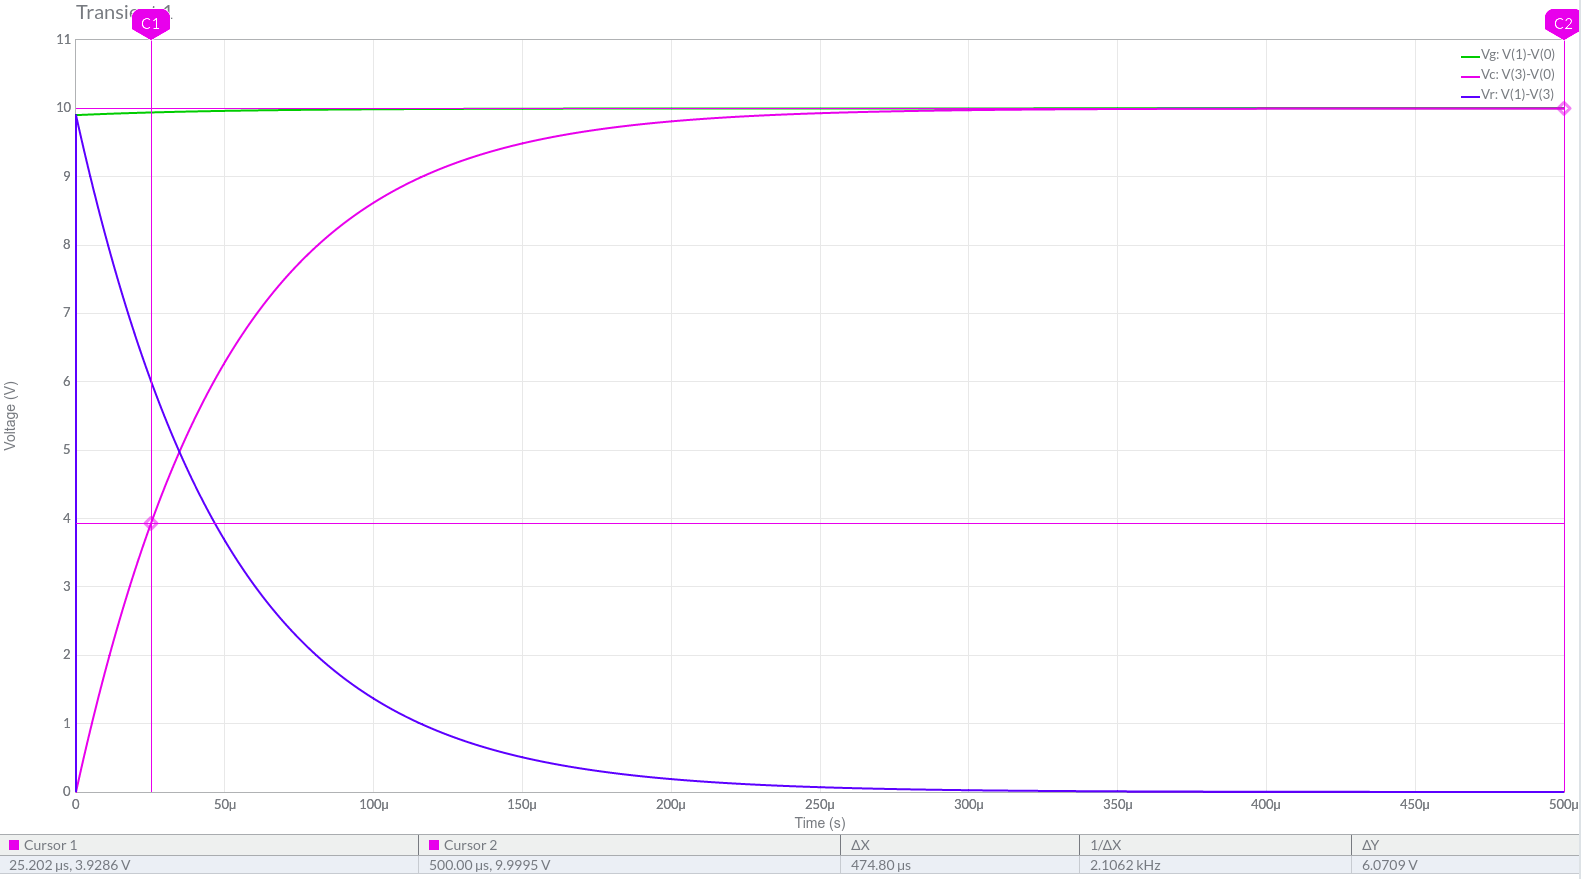
\includegraphics[width=\textwidth]{fig/1-c}
  \caption{Gráfico da simulação no domínio [0, T/2]. Cursor C1 marcando 25.202 $\mu$s em $x$ e 3.9286 V em $y$.}
\end{figure}

Da definição de logarítmo e da equação (6) da apostila teórica:

\begin{equation}
  \log_{b}a = x \;\; \Leftrightarrow \;\; b^{x} = a
\end{equation}

\begin{equation}
  v_{c}(t) = E(1 - e^{-\frac{t}{\uptau}}) \;\; \Rightarrow \;\; e^{-\frac{t}{\uptau}} = 1 - \frac{v_{c}}{E}
\end{equation}

\begin{flalign}
  (1) \Rightarrow (2): && \uptau &= -\frac{t}{\ln\left(1-\frac{v_{c}}{E}\right)}&
  \label{eq:tau}
\end{flalign}

Aplicando os valores $E = 10\ \text{V}$, $t = 25.202\ \mu\text{s}$ e $v_{c} = 3.9286\ \text{V}$ da simulação na equação \ref{eq:tau}, temos:

$$
  \uptau = 50.51\ \mu\text{s}
$$

\subsection*{Item 1.d}

$$
  R_{T} = R_{g} + R = (50 + 5 \cdot 10^{3})\ \Omega = 5.05\ \textnormal{k}\Omega
$$

$$
  \uptau = R_{T}C = (5.05 \cdot 10^{3}\ \Omega)(10 \cdot 10^{-9}\ \textnormal{F}) = 50.50\ \mu \textnormal{s}
$$

\begin{table}[h!]
  \centering
  \begin{tabular}{|c|c|c|c|}
    \hline
    Período do Sinal (T) & $\uptau$ (simulado) & $\uptau$ (calculado) & Diferença relativa \\
    \hline
    1 ms                 & 50.51 $\mu$s        & 50.50 $\mu$s         & 0.002 \%           \\
    \hline
  \end{tabular}
  \caption{Comparação dos valores teórico e simulado.}
\end{table}

\subsection*{Item 1.e}

$$
  V_{1} = 0.1 \cdot 10\ \text{V} = 1\ \text{V}; \qquad V_{2} = 0.9 \cdot 10\ \text{V} = 9\ \text{V}
$$

\begin{figure}[h!]
  \centering
  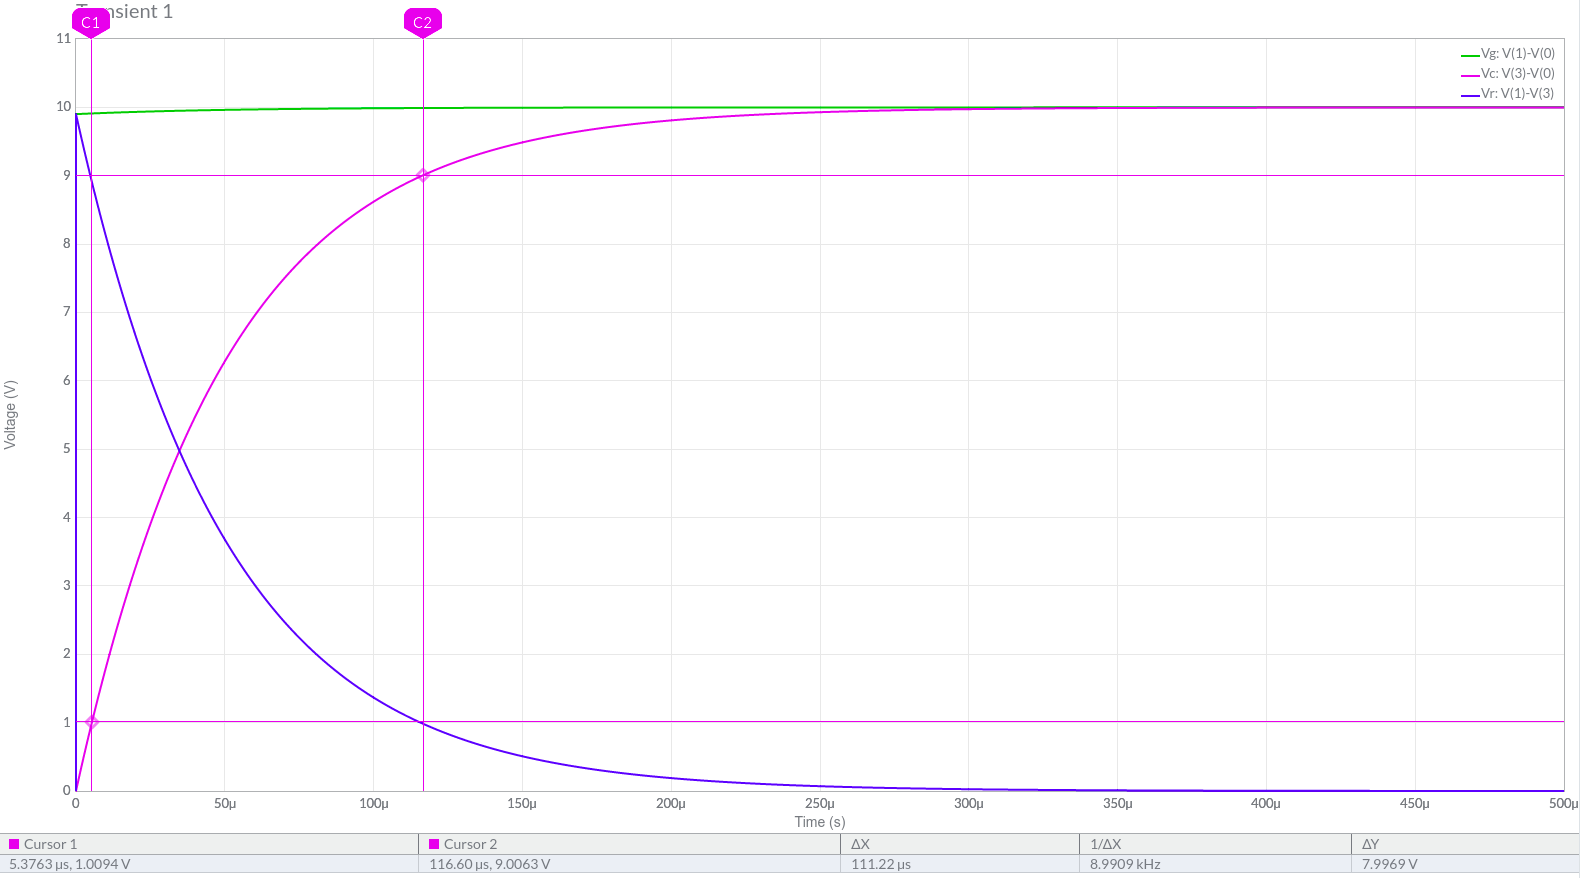
\includegraphics[width=\textwidth]{fig/1-e}
  \caption{Grádifo da simulação. Cursor C1 marcando 5.3763 $\mu$s em $x$ e 1.0094 mV em $y$ e cursor C2 marcando 116.60 $\mu$s em $x$ e 9.0063 V em $y$. $\Delta x$ = 111.22 $\mu$s}
\end{figure}

$$
  t_{r} = \Delta x = 111.22\ \mu\text{s}
$$

\pagebreak

\subsection*{Item 1.f}

\begin{figure}[h!]
  \centering
  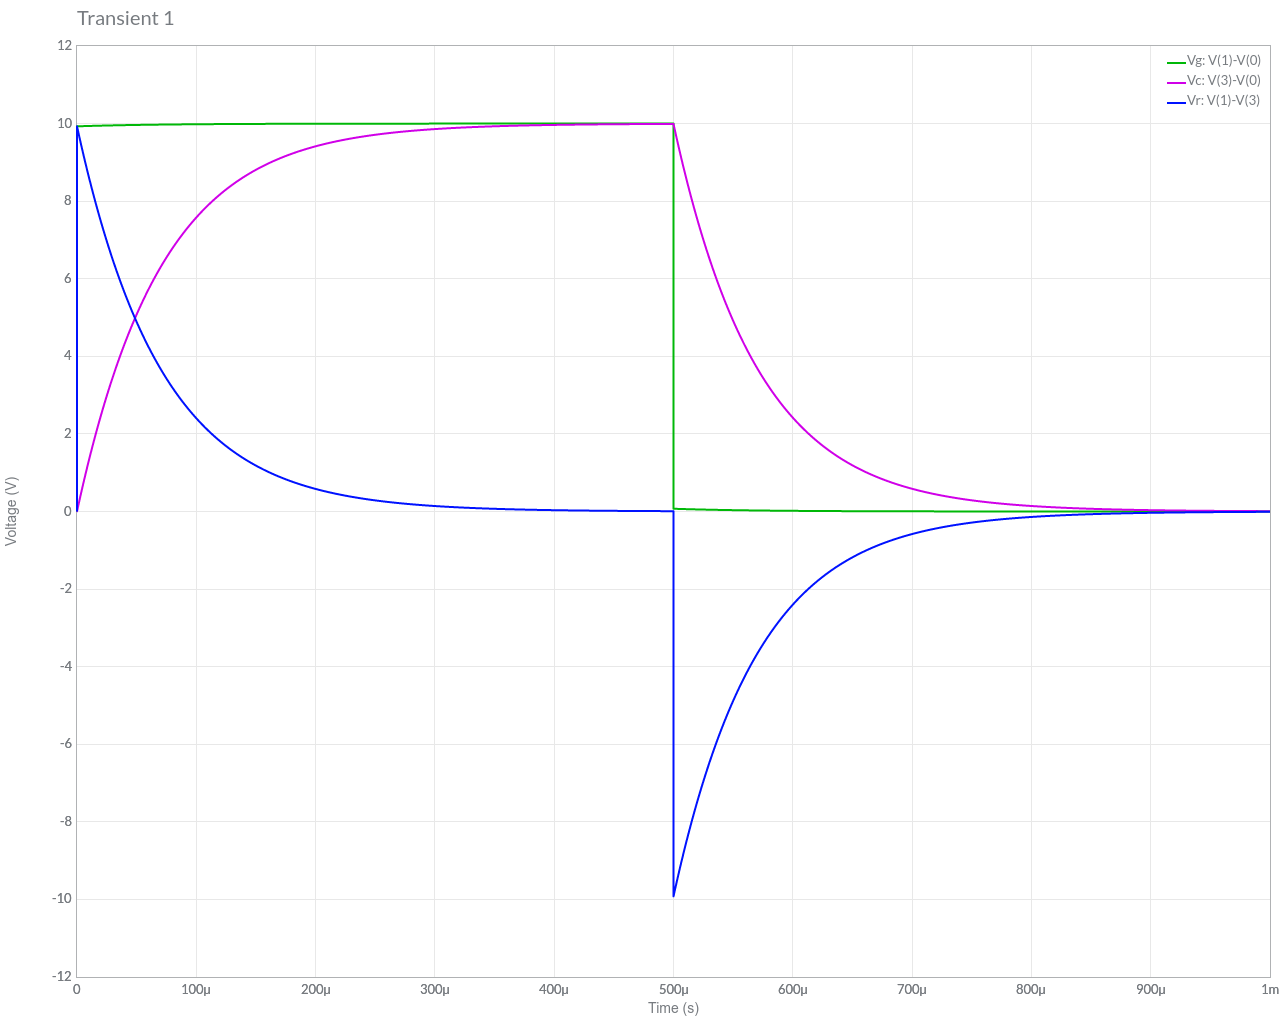
\includegraphics[width=.8\textwidth]{fig/1-p-70}
  \caption{Gráfico da simulação para resistência de 7 k$\Omega$ no potenciômetro.}
\end{figure}

\begin{figure}[h!]
  \centering
  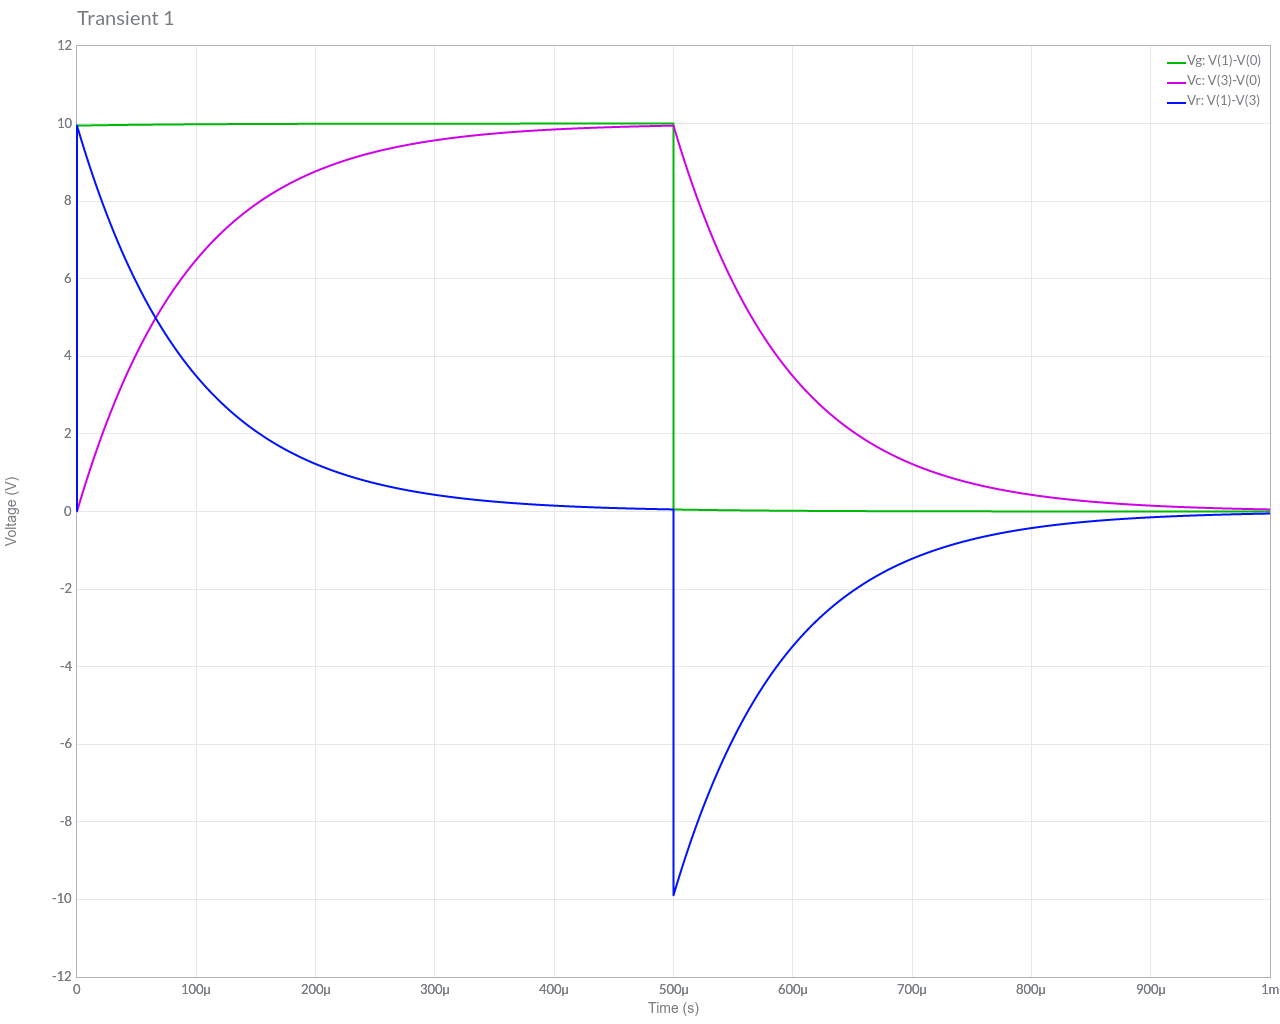
\includegraphics[width=.8\textwidth]{fig/1-p-95}
  \caption{Gráfico da simulação para resistência de 9.5 k$\Omega$ no potenciômetro.}
\end{figure}

\pagebreak

\subsection*{Item 2.a}

\begin{figure}[h!]
  \centering
  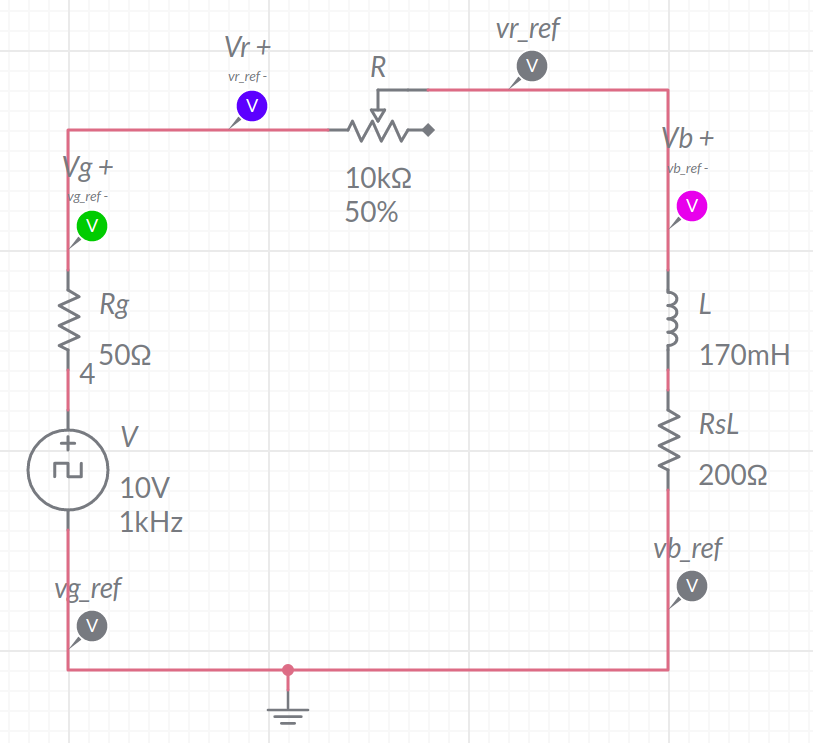
\includegraphics[width=.7\textwidth]{fig/2-circ}
  \caption{Esquema do circuito}
  \label{fig:2-circ}
\end{figure}

\begin{figure}[h!]
  \centering
  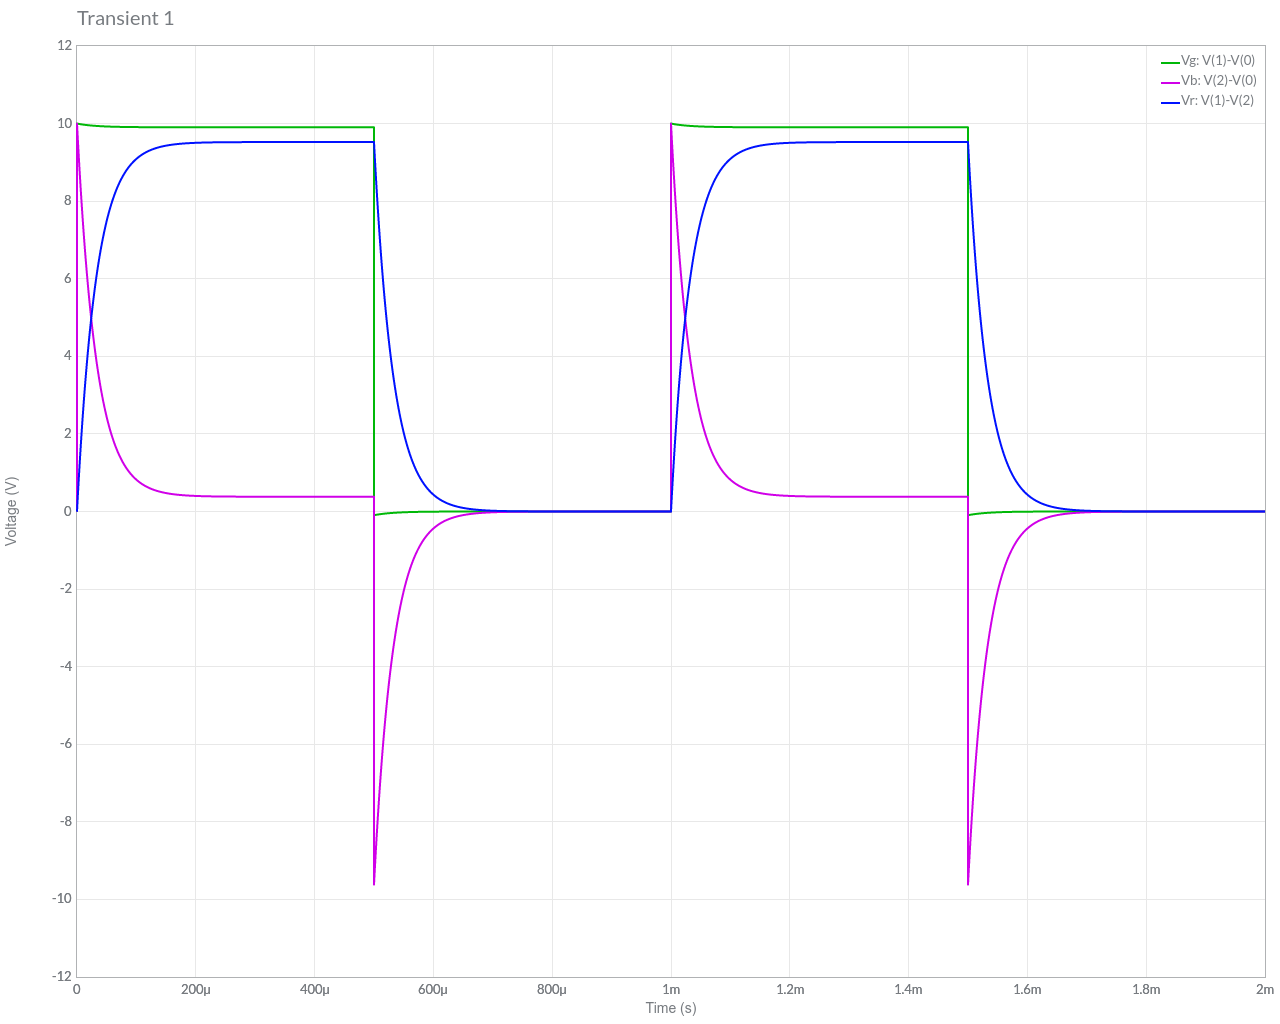
\includegraphics[width=.8\textwidth]{fig/2-sim}
  \caption{Simulação do circuito da figura \ref{fig:2-circ}}
  \label{fig:2-sim}
\end{figure}


\subsection*{Item 2.b}

As curvas de tensão no resistor (exponencial crescente) e na bobina (exponencial decrescente) vistas na simulação da figura \ref{fig:2-sim} apresentam uma forma coerente com a que se espera teoricamente.

$$
  V_{L}(t) = Ee^{-\frac{t}{\uptau}} \qquad V_{R}(t) = E(1 - e^{-\frac{t}{\uptau}})
$$

\subsection*{Item 2.c}

A curva de $V_{R}$ é invertida nos circuitos. No circuito RC, $V_{R}$ tende a zero para estabilizar durante o sinal alto do gerador. Já no circuito RL, o oposto é observado: $V_{R}$ tende ao sinal do gerador para se estabilizar.

\subsection*{Item 2.d}

\begin{figure}[h!]
  \centering
  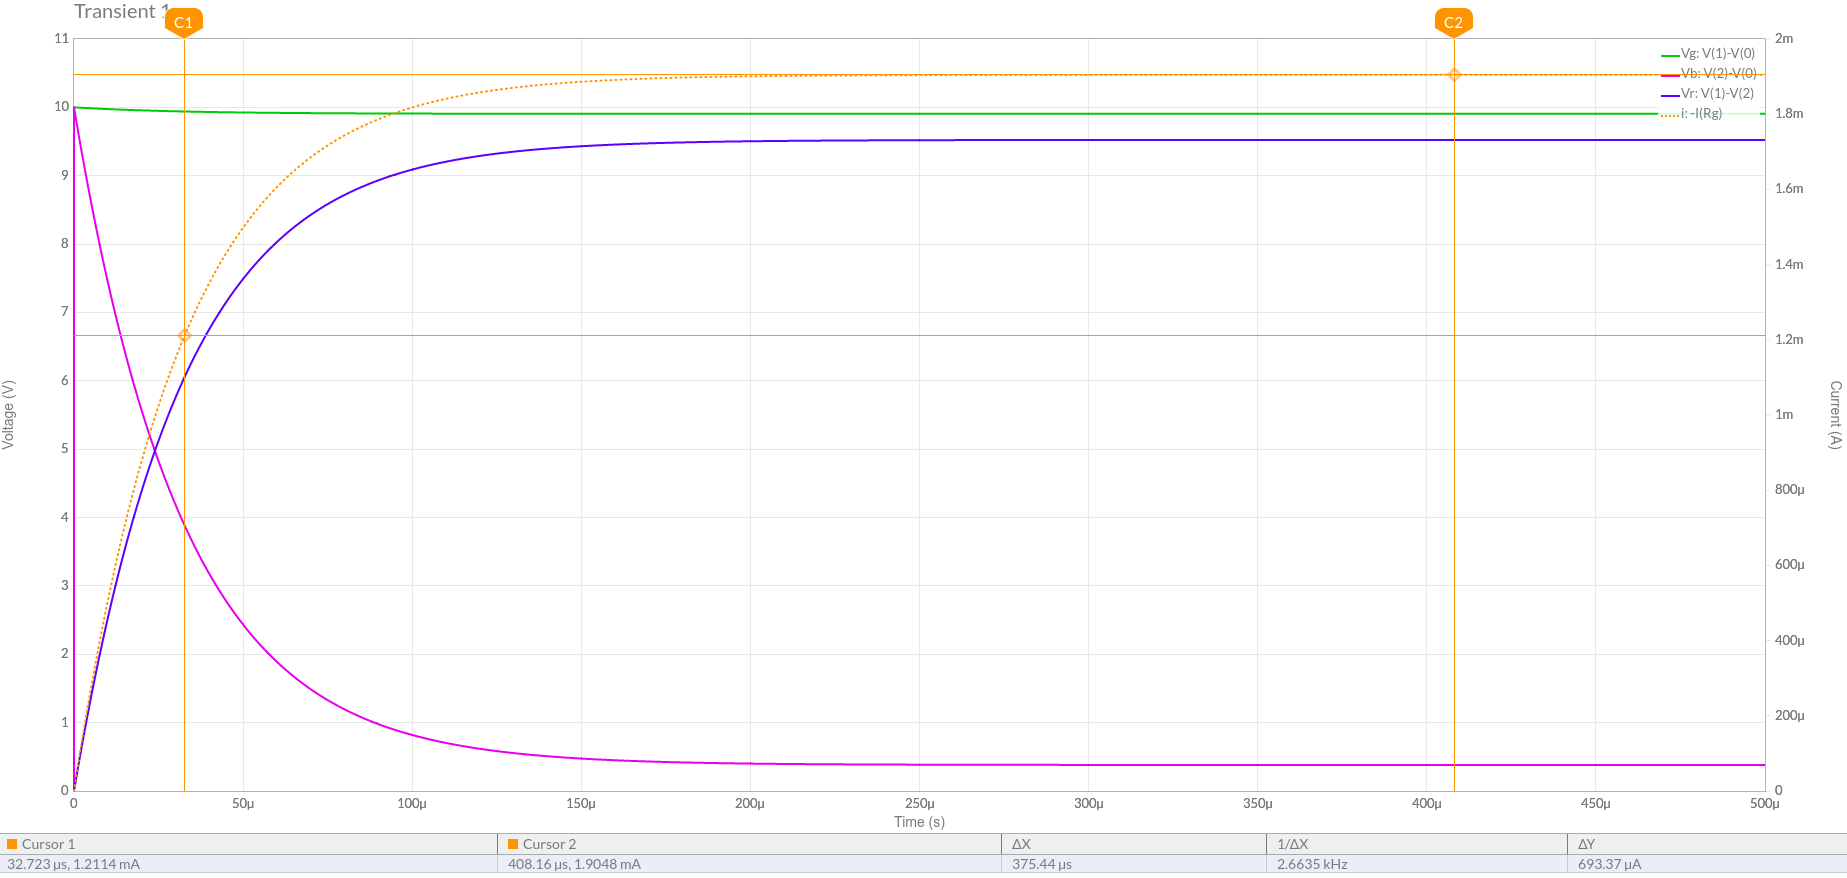
\includegraphics[width=\textwidth]{fig/2-d}
  \caption{Simulação do circuito com o gráfico da corrente em laranja. O cursor C1 indica o valor de 32.723 $\mu$s no eixo $x$ e 1.2114 mA no eixo $y$ e o cursor C2 indica o valor de 408.16 $\mu$s no eixo $x$ e 1.9048 mA no eixo $y$.}
  \label{fig:2-d}
\end{figure}

No instante $t = \uptau$, a corrente do circuito $i(t)$ está reduzida a uma fração $\frac{1}{e}$ do valor inicial. Assim,

$$
  i(t\!=\!\uptau) \:=\: \left( 1 - \frac{1}{e} \right) \cdot i_{o}
$$

Substituindo o valor da corrente do cursor C2 da figura \ref{fig:2-d}:

$$
  i(t\!=\!\uptau) \:=\: 1.21\ \text{mA}
$$

Portanto, pela medição do cursor C1, $\uptau$ = 32.72 $\mu$s.

\subsection*{Item 2.e}

Foi oberservado que, na subida, quanto maior o valor da resistência, mais rápida a curva $V_{R}$ se aproxima da tensão $V_{g}$ e, igualmente mais rápida, a curva $V_{b}$ se aproxima de zero. O parâmetro afetado foi a frequência de corte, pois o valor de $\uptau$ aumenta.

\pagebreak

\subsection*{Item 2.f}

\begin{figure}[h!]
  \centering
  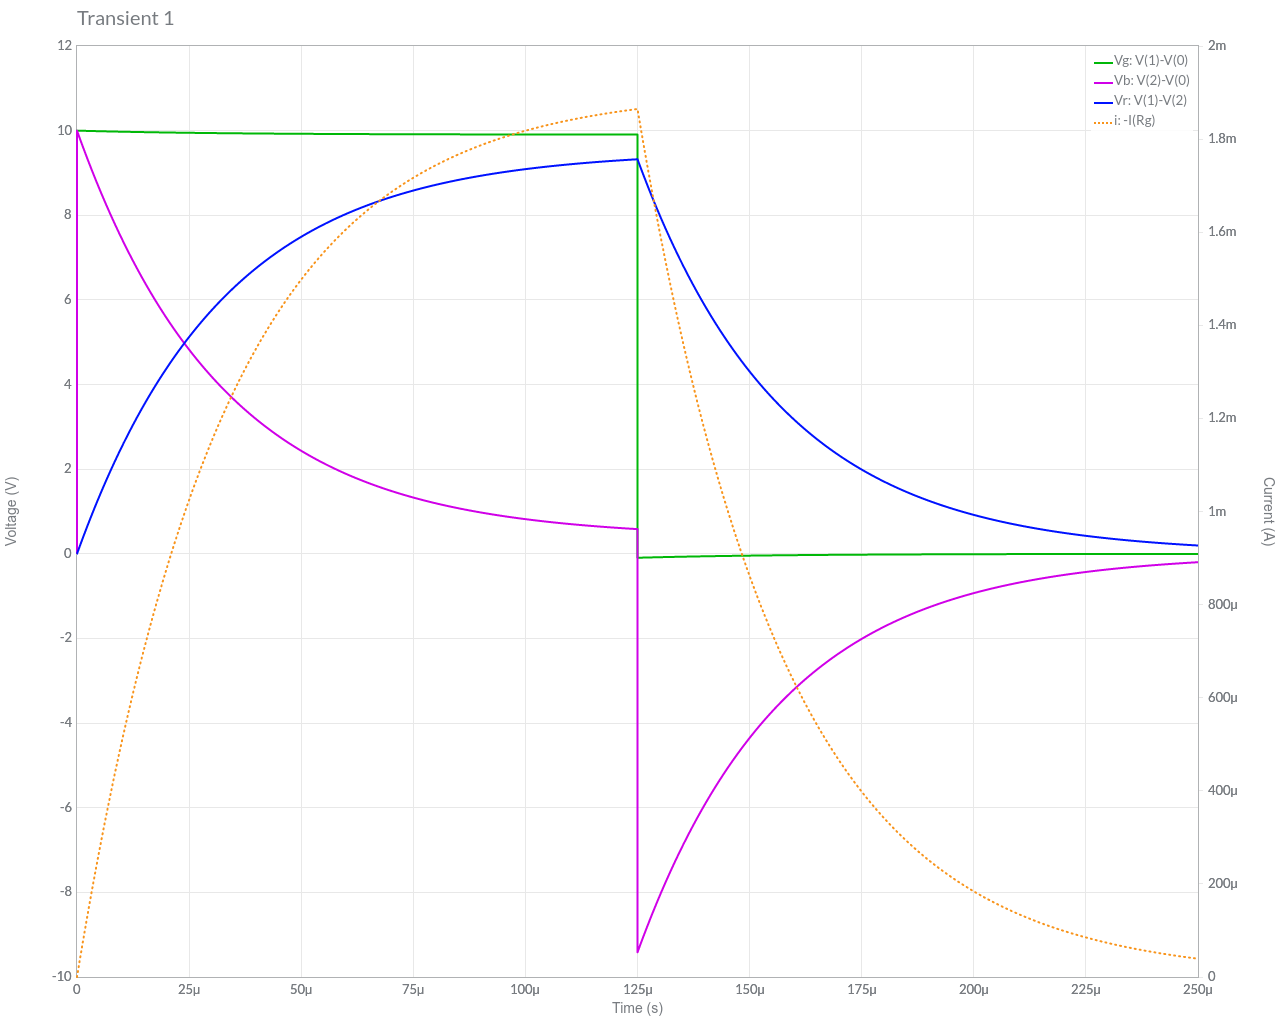
\includegraphics[width=.9\textwidth]{fig/2-f-4k}
  \caption{Simulação da tensão e corrente do circuito para resistência do potenciômetro igual a 4 k$\Omega$.}
  \label{}
\end{figure}

\begin{figure}[h!]
  \centering
  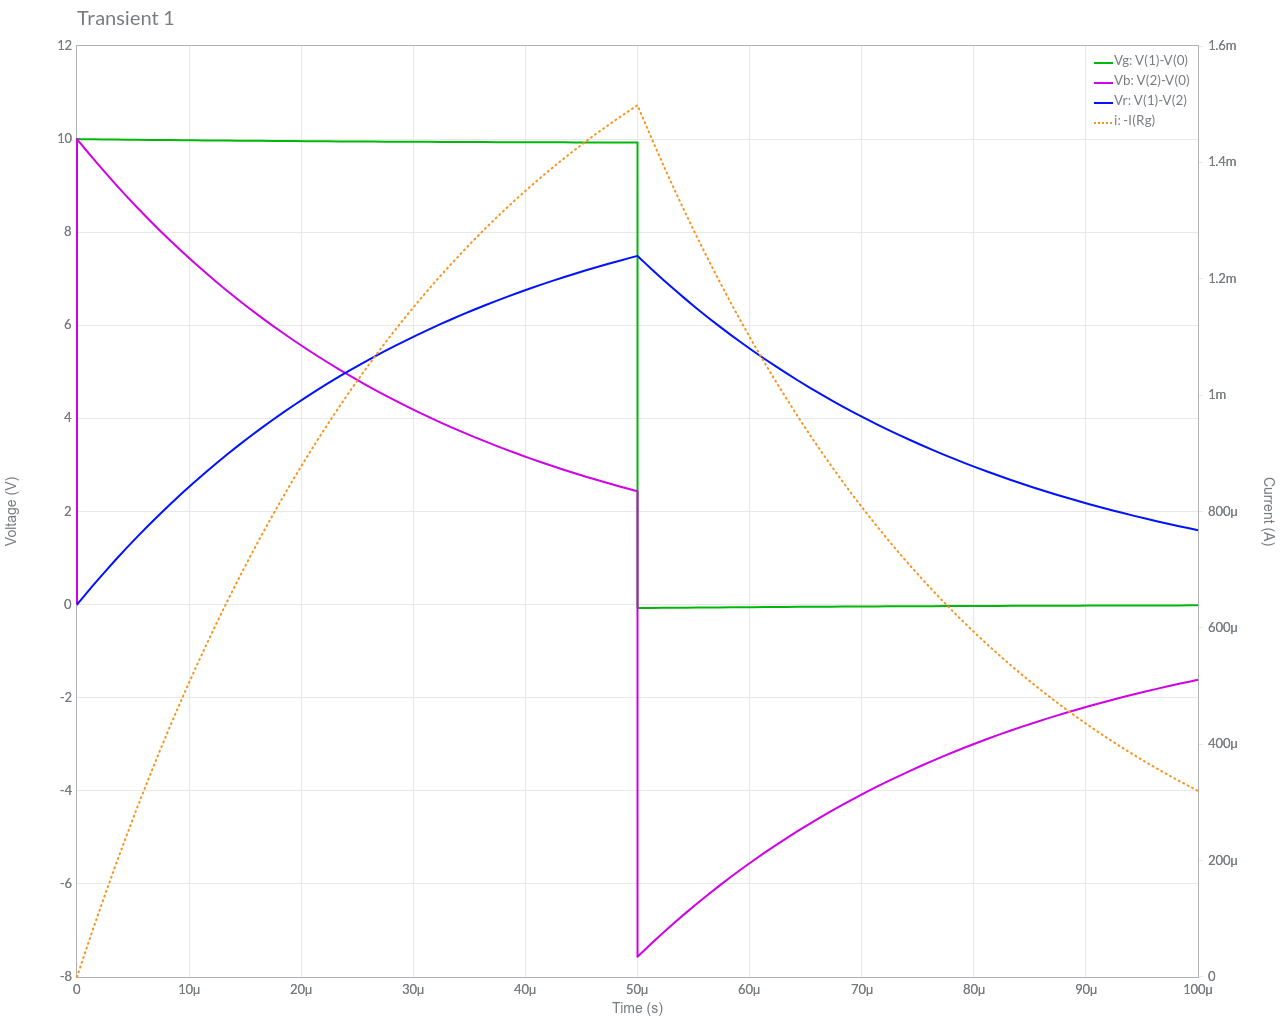
\includegraphics[width=.9\textwidth]{fig/2-f-10k}
  \caption{Simulação da tensão e corrente do circuito para resistência do potenciômetro igual a 10 k$\Omega$.}
  \label{}
\end{figure}

Neste experimento foi notado que quanto maior a frequência da onda quadrada que alimenta o circuto, mais a tensão de saída (capacitor) demora para atingir o valor de patamar antes da mudança de estado do sinal. Sendo que para frequências muito altas a curva nem chega a atingir o valor de patamar, pois, nestes casos, $\uptau \ll T/2$.

\end{document}
